\documentclass[11pt,a4paper]{article}
\usepackage[utf8]{inputenc}
\usepackage[english]{babel}
\usepackage{graphicx}
\usepackage{listings}
\begin{document}
\title{How do you make a strong passphrase?}
\author{Tom Eccles}
\maketitle

\section{Introduction}
I am writing this in response to repeated claims by some large news organisations that a good way of having a strong passphrase is to use as many different character types as possible (the example they gave was to use "pa\$\$word"\footnote{It is worth noting that using "leet speak" such as replacing "s" with "\$" or replacing "l" with "1" or "a" with "@" provides less security than one might expect because many modern brute forcing tools such as John The Ripper (http://www.openwall.com/john/) can automatically try "leet speak" variations to a given dictionary.} instead of "password". This in it's self I agree with, however they did not even mention the importance of passphrase length. In this document I hope to provide a simple mathematical argument for the importance of passphrase length. 

\section{Threat Model}
I will be discussing the case where an attacker is attempting to gain access to an account by trying every possible password until one works (a brute force attack). I am also assuming that the attacker is not targeting the user directly because in this case I believe that the majority of users have no chance at all due to the effectiveness of social engineering attacks such as spear phishing. 

\section{The Mathematics}
\subsection{Assumptions and Probability}
I am going to assume that the probability an attacker guessing one character in a passphrase is independent of them guessing another character. This may not be strictly true because the attacker may have some very intelligent software which (if the passphrase is composed of words) may be able to guess the remaining characters of a word after it already has some of them (like the child's game 'Hangman'). This assumption has been made to make the mathematics solvable with my knowledge. I think that this assumption is reasonable because we are discussing an attacker who is trying every possible passphrase.

As anyone who has studied probability knows, the probability of two independent events both occurring equals the product of the two events: $P(A \cap B)=P(A)P(B)$. And such follows for more independent events: they are all multiplied together.

%EDITEDThe other bit of probability which we will need is that (assuming a uniform random distribution across all characters in the passphrase\footnote{This is another assumption which may not be true if the attacker uses very intelligent software: the attacker may realise that alphabetical characters are more likely and so create an effect similar to a loaded die. However, as we are discussing the case were an attacker is brute forcing every possible passphrase, I believe that this is a reasonable assumption.}) with $n$ different characters, the probability $P$ of an individual character being chosen is $P = \frac{1}{n}$.

Therefore, if an attacker tries every password with a length of $n$ and a character space of $s$, the number of passwords which the attacker has tried is $s^n$.

However, in our threat model we specify that the attacker tries every password and so the attacker must try all of the lengths up to $n$ first. Therefore the number of attempts made by the attacker is $s + s^2 + s^3 +...+s^n$. This is similar to the geometric\footnote{see https://en.wikipedia.org/wiki/Geometric\_series} series $1 + s + s^2 +...+s^n$, which (assuming that $s \ne 1$) has a sum equal to \[\frac{s^n - 1}{s-1}\]This is geometric series is 1 too high for us and so the sum of all the attempts made by the attacker is \[\frac{s^n - 1}{s-1} -1\]I will refer to this as the complexity of the passphrase, $c$. This inherits the same constraint that $s \ne 1$. This does not matter because the character space will always be greater than 1.

\subsection{Rates of Change}
In this section I will try to demonstrate algebraically that the increase in passphrase complexity due to length is more rapid than the increase due to the character space. 

The rate of change of complexity with respect to the length of the passphrase while keeping the character space constant (the partial differential of complexity with respect to length) is \[ \frac{\partial c}{\partial n} = \frac{s^n ln(s)}{s-1}\]

The rate of change of complexity with respect to the character space (the partial differential of complexity with respect to character space) is \[ \frac{\partial c}{\partial s} = \frac{ns^{n-1}-s^n+1}{(s-1)^2}\]

While it is difficult to see which is larger by inspection, a Wolfram-Alpha\footnote{Wolfram-Alpha is a knowledge engine capable of (amongst other things) investigating inequalities. See http://www.wolframalpha.com/} computation of \[\frac{ns^{n-1}-s^n+1}{(s-1)^2} < \frac{s^n ln(s)}{s-1}\]

Shows solutions for most positive values of $s$ and $n$.\footnote{I am unable to reproduce the inequality plot here because I do not have a Wolphram-Alpha Pro account.} The only exception to this is for very small values (less than 5) of $s$ and large values of $n$. However this is not important because almost everyone includes alphabetical characters in their passwords and just this puts us far into the realm of possible solutions when discussing reasonable values for $n$. Therefore, I conclude that for passphrases within our threat model, the increase in complexity is greater for increasing the length of the passphrase than for increasing the character space.

\subsection{A Graphical Method}
In case you do not want to type that long inequality into Wolfram-Alpha, I have also drawn a graph that shows (although not as clearly as I would have liked) that there is a faster increase of complexity with the length of the passphrase than with the size of the character space (note: when complexity becomes very high, this cannot be shown on the graph, this is why there is a blank section for larger values of $s$ and $n$):

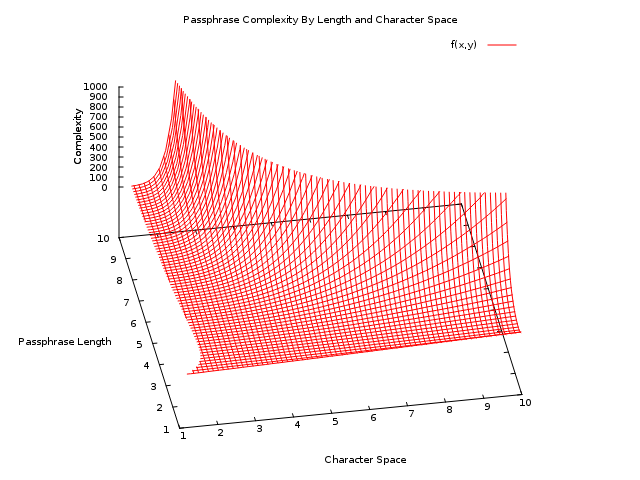
\includegraphics[scale=0.6]{graph1.png}
\pagebreak

And from the top looking down:

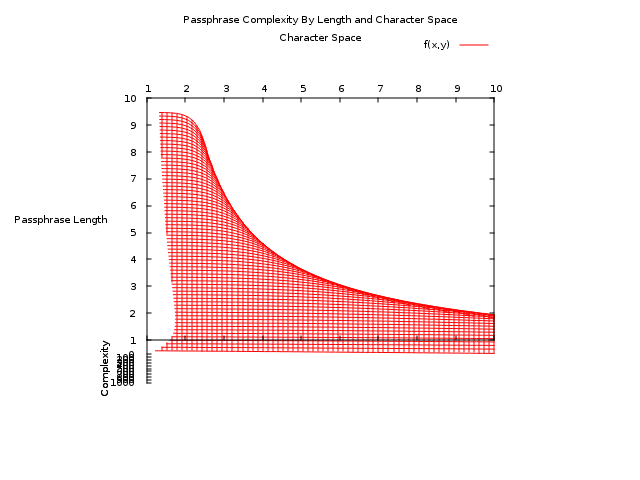
\includegraphics[scale=0.8]{graph2.png}

\section{Conclusion}
In conclusion I have shown that it is important to have both a long passphrase and several types of characters. Although it is worth noting that just by having lower and upper case characters, you already have a character space of 48. So my advice would be to concentrate on increasing the length of your passphrases. A good way of doing this is to use several words which do not make grammatical sense together. For a good explanation see https://xkcd.com/936/.

\pagebreak
\section{Appendices}
\subsection{"Passphrase?"}
I have chosen to use the word "passphrase" over the word "password" because it encourages longer login identifiers. There is no reason to use a single word and this should be discouraged as it is easier to brute force.

\subsection{Why are you just referencing a Wolfram Alpha?}
If you can show this mathematically then please contact me as I would be very interested to see how you did it. I was unable to.

\subsection{GNU-Plot Script to plot the graphs}
To display the graphs using gnu-plot (http://gnuplot.info/) on GNU+Linux run the following:
\begin{lstlisting}
gnuplot -p gnuplot1.txt
gnuplot -p gnuplot2.txt
\end{lstlisting}
Where there is a file in your current working directory called "gnuplot1.txt" containing the following:
\begin{lstlisting}
# titles
set title "Passphrase Complexity By Length and Character Space
set xlabel "Character Space"
set ylabel "Passphrase Length"
set zlabel "Complexity" rotate by 90

# look pretty
set isosamples 70
set samples 60

# ranges
set xrange[1:10]
set yrange[1:10]
set zrange[1:1000]

# set viewing angle
set view 38, 350

# plot it
f(x,y) = (((x**y)-1)/(y-1))-1
splot f(x,y)
\end{lstlisting}
And a file called "gnuplot2.txt" containing the following:
\begin{lstlisting}
# titles
set title "Passphrase Complexity By Length and Character Space
set xlabel "Character Space"
set ylabel "Passphrase Length"
set zlabel "Complexity" rotate by 90

# look pretty
set isosamples 70
set samples 60

# ranges
set xrange[1:10]
set yrange[1:10]
set zrange[1:1000]

# set viewing angle
set view 350, 0

# plot it
f(x,y) = (((x**y)-1)/(y-1))-1
splot f(x,y)
\end{lstlisting}

For usage on other platforms refer to the gnu-plot documentation for your platform or enter the gnu-plot commands listed above manually into a gnu-plot shell.

\subsection{Distribution and Licensing}
This work is distributed under  Creative Commons Attribution-ShareAlike 4.0 International (see https://creativecommons.org/licenses/by-sa/4.0/).

\end{document}